\documentclass[11pt]{beamer}
\usepackage[T1]{fontenc}
\usepackage{lmodern}
\usepackage{amsmath}
\usepackage{amsfonts}
\usepackage{amssymb}
\usepackage{graphicx}
\usetheme{Madrid}
\usepackage{marvosym,graphicx,subfloat,subfig,tikz}

\usepackage{graphicx} 
\newcommand\mybox[2][]{%
\tikz[overlay]\node[inner sep=2pt, anchor=text, rectangle, rounded corners=1mm,#1] {#2};% 
\phantom{#2}}
\usefonttheme[onlylarge]{structurebold}
\setbeamerfont*{frametitle}{size=\normalsize,series=\bfseries}
\setbeamertemplate{navigation symbols}{}
\usepackage[english]{babel}
\usepackage[latin1]{inputenc}
\usepackage{times}
\usepackage{graphicx}
\usepackage[normalem]{ulem}
\usepackage{etex}
\usepackage{colortbl,booktabs}
\usepackage{tabularx}
\usepackage{float}
\usepackage{tikz}
\usepackage{multicol}

\begin{document}
	\author[Harish, Ankit, Bhushan, Vineet, Karthikeya]{Harish(55)
		Ankit(41)
		Bhushan(59)\\
		Vineet(46)
		Karthikeya(32)
	}
	\title[Musical Instrument Classification]{\textbf{
			Predominant Musical Instrument Classification based
			on Spectral Features} \vspace*{3pt}}
	%\subtitle{}
	%\logo{}
	%\institute{}
	\institute[]{\small Indian Statistical Institute}
	\date[November 25, 2019]{\small CDS Course Project Presentation \\ November 25, 2019}
	%\subject{}
	%\setbeamercovered{transparent}
	%\setbeamertemplate{navigation symbols}{}
	\begin{frame}[plain]
		\maketitle
	\end{frame}
	
	\begin{frame}
		\frametitle{Musical Information Retrieval}
		Music information retrieval (MIR) is the interdisciplinary science of retrieving information from music.
		\pause
		\begin{block}{Key areas in MIR}
	 \begin{multicols}{2}
	 \begin{itemize}
	 \item Recommender Systems \item Track separation \item Genre Detection
	 \end{itemize}
	 \columnbreak\pause 
	 \begin{itemize}
	 \item Music Transcription \item Music Categorization \item Music Generation
	 \end{itemize}
	 \end{multicols}\pause
\begin{center}
\mybox[fill=green!30]{Musical Instrument Recognition}
\end{center}
		\end{block}
	\end{frame}
		\begin{frame}
		{Musical Instrument Classification}
		
		\begin{figure}
			\centering
			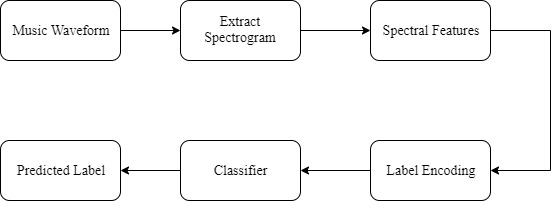
\includegraphics[width=0.7\linewidth]{Flowchart}
			\caption{Workflow for Musical Instrument Identification}
			\label{fig:flowchart}
		\end{figure}
		
	\end{frame}
	
	\begin{frame}
		{Dataset}
		
		\begin{figure}
			\centering
			
\includegraphics[width=0.2\linewidth]{IRMAS}
			%\caption{}
			\label{fig:irmas}
		\end{figure}
\begin{center}
		annotated polyphonic dataset\footnote{Janer \textit{et al.} ISMIR 2012} with predominant musical instrument
\end{center}
	\begin{figure}
		\centering
		
\includegraphics[width=0.6\linewidth]{irm-upf}
	\end{figure}\pause
		\begin{block}{Instruments}
			cello, clarinet, \mybox[fill=green!30]{flute}, \mybox[fill=green!30]{acoustic guitar}, electric guitar, \mybox[fill=green!30]{organ}, \mybox[fill=green!30]{piano}, saxophone, \mybox[fill=green!30]{trumpet}, violin, and \mybox[fill=green!30]{human voice}
		\end{block}
	
	
	\end{frame}
\begin{frame}{Dataset}
	\begin{figure}
		\centering
		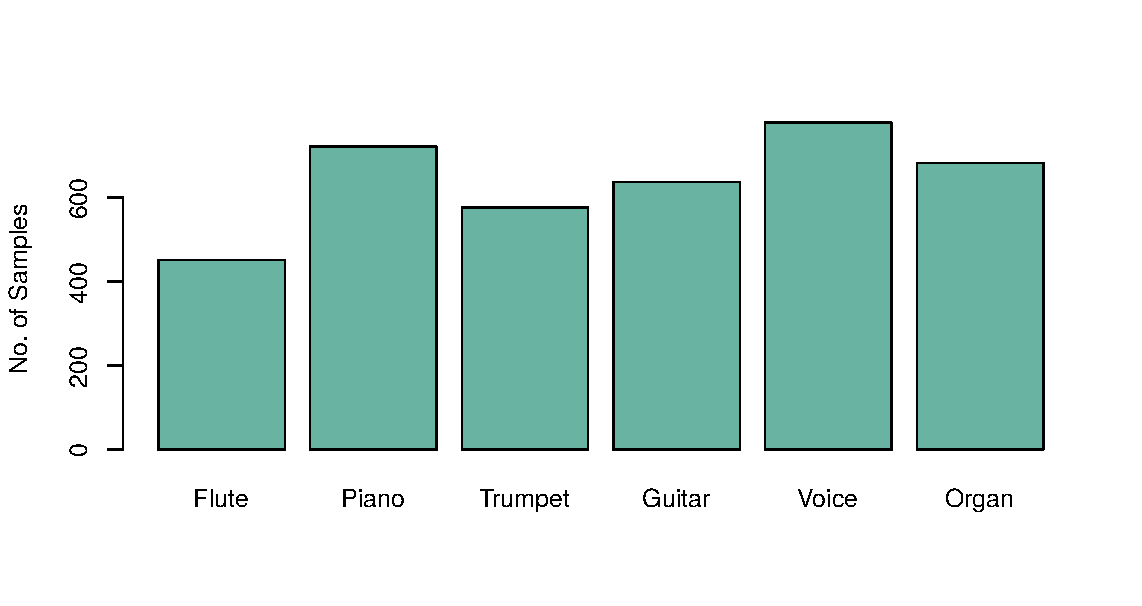
\includegraphics[width=0.8\linewidth]{instrument-hist}
		\caption{Number of audio samples per instrument class}
		\label{fig:instrument-hist}
	\end{figure}
\begin{center}
		Total \mybox[fill=green!30]{3 hr 12 min} of Audio Samples
\end{center}
\end{frame}
	
	\begin{frame}
		%Spectral Features\\
		\begin{block}{Timbre}
			Timbre is the `colour' of a sound. Timbre can distinguish between different types of string instruments, wind instruments, and percussion instruments.
		\end{block}
		\begin{figure}[!htb]
			\centering
			\subfloat[EDM ]{\label{fig:edm}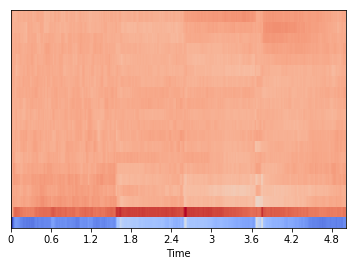
\includegraphics[width=25mm]{EDM.png}}
			\subfloat[Guitar (Accoustic) ]{\label{fig:gac}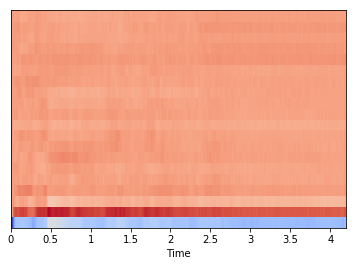
\includegraphics[width=25mm]{Guitar.png}}
			\\
			\subfloat[Key Board ]{\label{fig:key}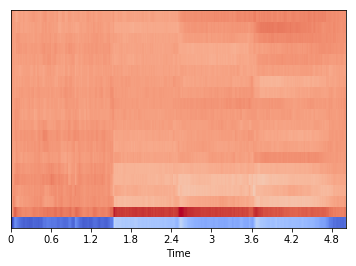
\includegraphics[width=25mm]{keyboard.png}}
			\subfloat[Organ ]{\label{fig:org}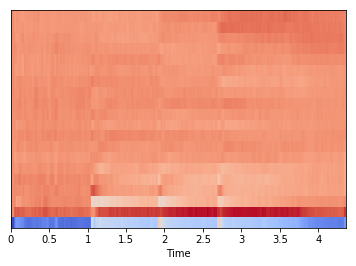
\includegraphics[width=25mm]{Organ.png}}
			\caption{Same note (audio) played on various instruments}
			\label{fig:instr}
		\end{figure}
	\end{frame}
	\begin{frame}
		{MFCC Calculation Flowchart}
		\begin{figure}
			\centering
			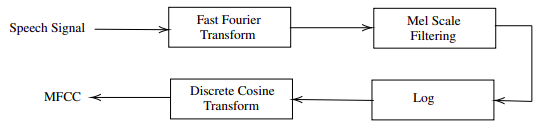
\includegraphics[width=0.7\linewidth]{mfcc}
			\caption{MFCC Calculation Workflow}
			\label{fig:mfcc}
		\end{figure}
		
		\pause
		\begin{figure}
			\centering
			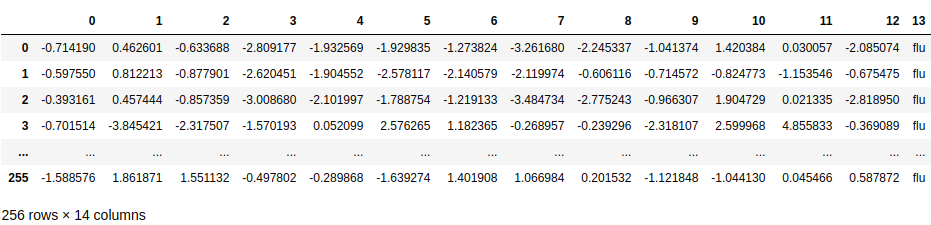
\includegraphics[width=0.8\linewidth]{mfcc-features}
			\label{fig:mfcc-features}
		\end{figure}
	
	\begin{center}
		\texttt{np.mean(mfcc-feature-vector,axis=1)}
	\end{center}
	\pause
	\begin{figure}
		\centering
		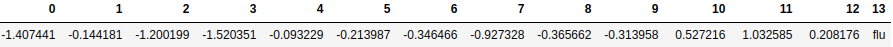
\includegraphics[width=0.8\linewidth]{fv}
	\end{figure}
		
	\end{frame}

	\begin{frame}
	{Other Spectral Features}	 %\cite{Eronen2000}
	
	\begin{itemize}
		\item Zero Crossing Frequency --- simple measure of the frequency content of a signal
	\item Root mean Square --- rms summarises the energy distribution of each frame
	\item Spectral Centroid --- It is a measure of average frequency weighted by the sum of spectral amplitude within one frame
	\item Spectral Bandwidth --- frequency range of a signal weighted by its spectrum
	\item Spectral Rolloff --- measure of rolloff frequency
	
	\end{itemize}
\end{frame}


\begin{frame}{Methodology}
	\begin{itemize}
		\item We experimented with two libraries -- Essentia \& Librosa for feature extraction
		\item Each audio sample of 3 sec produced 257 rows. We took mean and produced a single vector per audio file
		\item Labelled each vector using \texttt{labelencoder}
		\item trained the classifier in \texttt{scikit learn}
		
	\end{itemize}
	
	
\end{frame}
	
\begin{frame}{Supervised Classification}
	\begin{itemize}
		\item Logistic Regression --- (Baseline Model)
		\item Decision Tree 
	\item LGBM 
	\item XG Boost 
	\item Random Forest 
	\item Support Vector Machine
	\end{itemize}
\end{frame}





\begin{frame}{Model Evaluation}
	
	
	\begin{itemize}
		\item \mybox[fill=green!30]{Precision} is the ratio $\frac{tp}{(tp + fp)}$ where $tp$ is the number of true positives and $fp$ the number of false positives. The precision is intuitively the ability of the classifier not to label as positive a sample that is negative. 
		\pause
		
		\item \mybox[fill=green!30]{Recall} is the ratio  $\frac{tp}{(tp + fn)}$ where $tp$ is the number of true positives and $fn$ the number of false negatives. The recall is intuitively the ability of the classifier to find all the positive samples. 
		
		\pause
		\item \mybox[fill=green!30]{F1 score} can be interpreted as a weighted average of the precision and recall. $$F1 = \frac{2 \times (\rm{precision} * \rm{recall})}{ (\rm{precision} + \rm{recall})}$$
		\pause
		\item \mybox[fill=green!30]{Confusion Matrix} is a technique to evaluate performance of a supervised classification. Calculating a confusion matrix gives a better idea of what our classification model is getting right and what types of errors it is making.
		\end{itemize}
	
\end{frame}

\begin{frame}{Accuracy Statistic}
	\begin{minipage}{8cm}
			\begin{center}\scriptsize
			\begin{table}[h!]
				\begin{tabular}{@{}l|lll|lll|lll@{}}
					\toprule
					& \multicolumn{3}{c}{\textbf{Logistic Regession}}                        & \multicolumn{3}{c}{\textbf{Decision Tree}}                             & \multicolumn{3}{c}{\textbf{LGBM}}                                      \\ \midrule
					Instrument & \multicolumn{1}{c}{P} & \multicolumn{1}{c}{R} & \multicolumn{1}{c}{F1} & \multicolumn{1}{c}{P} & \multicolumn{1}{c}{R} & \multicolumn{1}{c}{F1} & \multicolumn{1}{c}{P} & \multicolumn{1}{c}{R} & \multicolumn{1}{c}{F1}\\ 
					Flute      & 0.58                  & 0.39                  & 0.47                   & 0.43                  & 0.44                  & 0.43                   & 0.66                  & 0.59                  & 0.62                   \\
					Piano      & 0.55                  & 0.59                  & 0.57                   & 0.53                  & 0.54                  & 0.53                   & 0.69                  & 0.73                  & 0.71                   \\
					Trumpet    & 0.44                  & 0.53                  & 0.48                   & 0.50                  & 0.46                  & 0.48                   & 0.59                  & 0.67                  & 0.63                   \\
					Guitar     & 0.63                  & 0.57                  & 0.60                   & 0.60                  & 0.57                  & 0.58                   & 0.73                  & 0.68                  & 0.71                   \\
					Voice      & 0.58                  & 0.48                  & 0.52                   & 0.52                  & 0.50                  & 0.51                   & 0.72                  & 0.54                  & 0.62                   \\
					Organ      & 0.51                  & 0.61                  & 0.56                   & 0.50                  & 0.55                  & 0.52                   & 0.63                  & 0.74                  & 0.68                   \\ 
				\end{tabular}
				
				
				\begin{tabular}{@{}l|lll|lll|lll@{}}
					\toprule
					& \multicolumn{3}{c}{\textbf{XG Boost}}                                  & \multicolumn{3}{c}{\textbf{RF}}                                        & \multicolumn{3}{c}{\textbf{SVM}}                                       \\ \midrule
					Instrument & \multicolumn{1}{c}{P} & \multicolumn{1}{c}{R} & \multicolumn{1}{c}{F1} & \multicolumn{1}{c}{P} & \multicolumn{1}{c}{R} & \multicolumn{1}{c}{F1} & \multicolumn{1}{c}{P} & \multicolumn{1}{c}{R} & \multicolumn{1}{c}{F1} \\
					Flute      & 0.66                  & 0.59                  & 0.62                   & 0.72                  & 0.48                  & 0.58                   & 0.63                  & 0.63                  & 0.63                   \\
					Piano      & 0.72                  & 0.71                  & 0.71                   & 0.72                  & 0.75                  & 0.74                   & 0.79                  & 0.84                  & 0.81                   \\
					Trumpet    & 0.58                  & 0.69                  & 0.63                   & 0.61                  & 0.72                  & 0.66                   & 0.78                  & 0.77                  & 0.78                   \\
					Guitar     & 0.71                  & 0.72                  & 0.71                   & 0.73                  & 0.72                  & 0.72                   & 0.77                  & 0.76                  & 0.77                   \\
					Voice      & 0.75                  & 0.53                  & 0.62                   & 0.74                  & 0.54                  & 0.62                   & 0.78                  & 0.67                  & 0.72                   \\
					Organ      & 0.65                  & 0.74                  & 0.69                   & 0.63                  & 0.80                  & 0.70                   & 0.79                  & 0.85                  & 0.82                   \\ \bottomrule
				\end{tabular}
				\vspace{0.1 in }
					\caption{Precision, Recall \& F1 Score for  various Supervised Models}
			\end{table}
		\end{center}
	\end{minipage}
\end{frame}	


\begin{frame}{Model Evaluation -- F1 Score}
	
	\begin{figure}
		\centering
		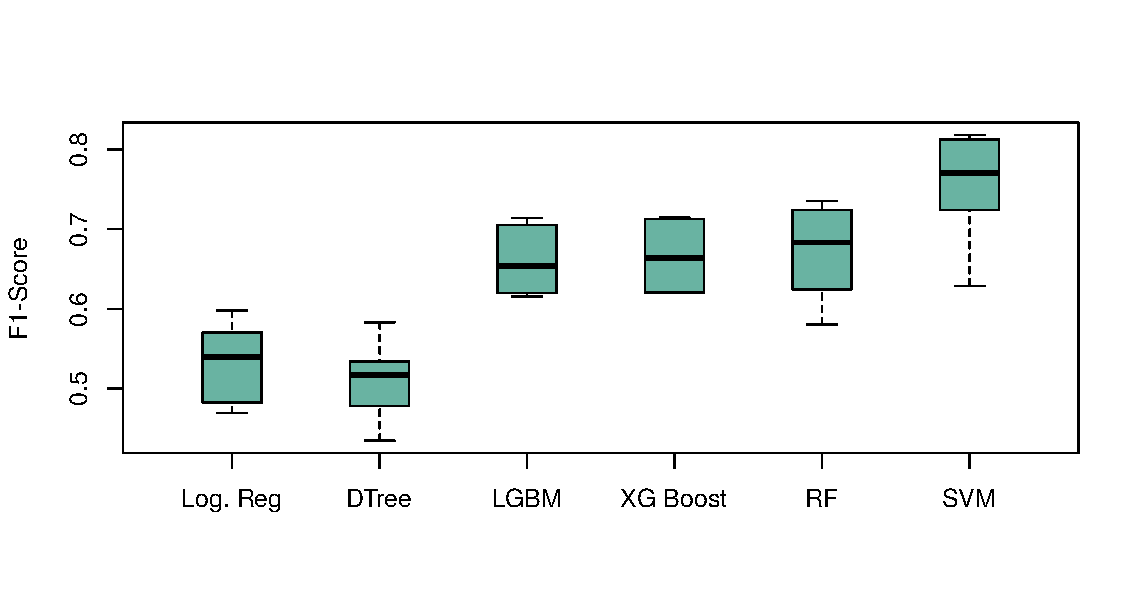
\includegraphics[width=\linewidth]{f1}
		\caption{F1 Measure for Various Models}
		\label{fig:f1}
	\end{figure}
\end{frame}


\begin{frame}{Instrument Performance}
	
	\begin{figure}
		\centering
		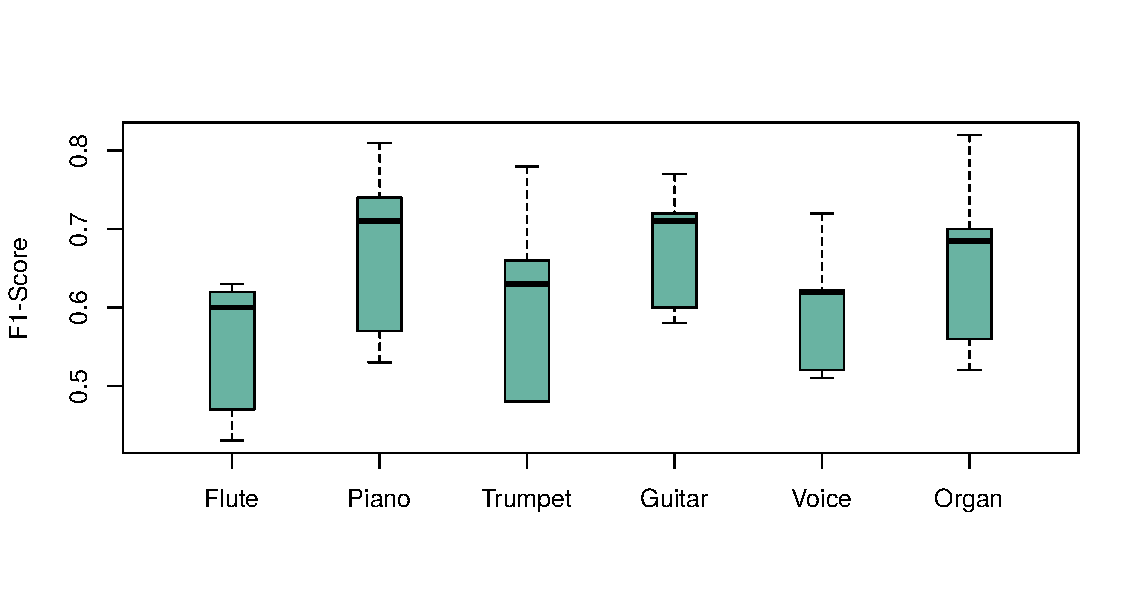
\includegraphics[width=0.95\linewidth]{instr-f1}
		\caption{Instrument wise classification}
		\label{fig:instr-f1}
	\end{figure}
	
	
\end{frame}



\begin{frame}{Model Evaluation -- Confusion Matrix}
	 
	 \begin{figure}[htp]
	 	\centering
	 	\subfloat[Logistic Regression ]{\label{figur:1}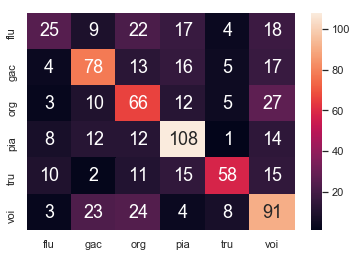
\includegraphics[width=40mm]{LogRegNew.png}}
	 	\subfloat[Decision Tree ]{\label{figur:2}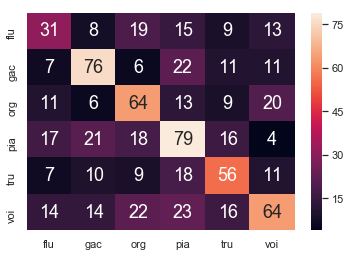
\includegraphics[width=40mm]{DecTreeNew.png}}
	 	\subfloat[Light GBM ]{\label{figur:3}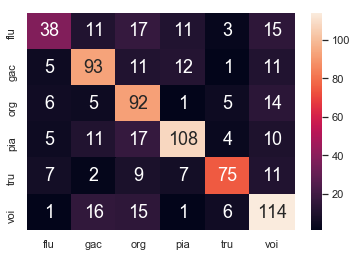
\includegraphics[width=40mm]{LGBMNew.png}}
	 	
	 	\caption{Confusion Matrix for various supervised Algorithms}
	 	\label{figur}
	 	
	 \end{figure}
	 
	 
\end{frame}

\begin{frame}{Model Evaluation -- Confusion Matrix}
	\begin{figure}[htp]
		\centering
		\subfloat[XG Boost ]{\label{figur:4}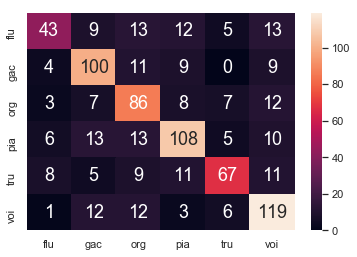
\includegraphics[width=40mm]{XGBoostNew.png}}
		\subfloat[Random Forest ]{\label{figur:5}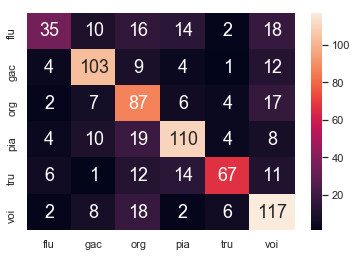
\includegraphics[width=40mm]{RandomForestNew.png}}
		\subfloat[SVM  ]{\label{figur:6}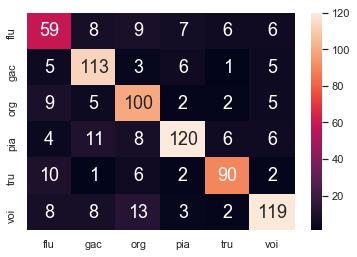
\includegraphics[width=40mm]{SVM_new.png}}
		\caption{Confusion Matrix for various supervised Algorithms}
		\label{figur2}
		
	\end{figure}
\end{frame}


\begin{frame}{Unsupervised Approach}
	\begin{multicols}{2}
		K-means Clustering
		 
		\columnbreak
		Hierarchical Clustering
\end{multicols}
\end{frame}

\begin{frame}{NN Arch}
	 \begin{figure}
	 	\centering
	 	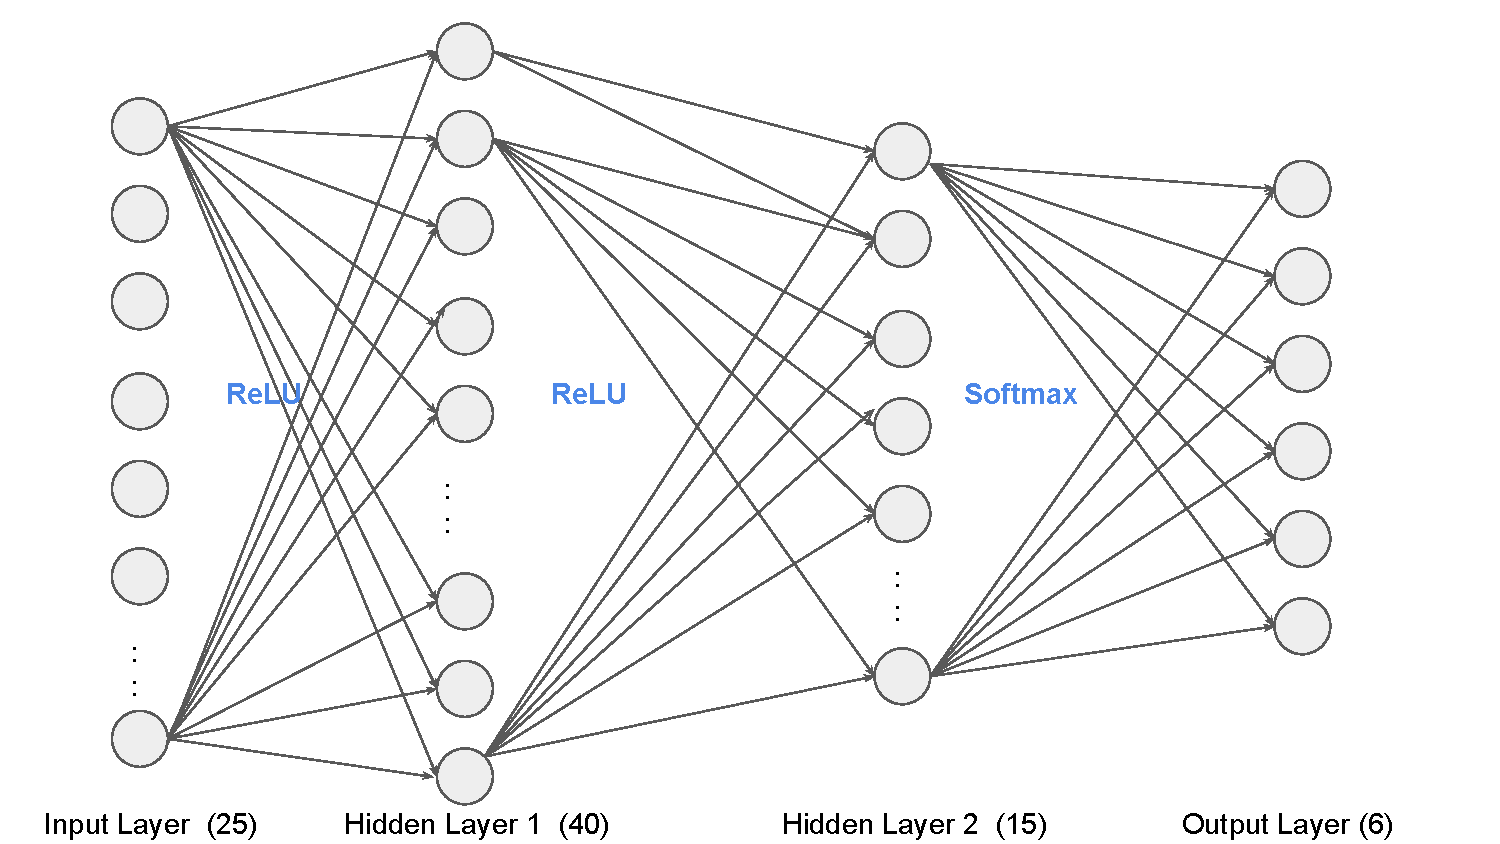
\includegraphics[width=0.85\linewidth]{nn.pdf}
	 	\caption{3 Layer Neural Network}
	 	\label{fig:nn}
	 \end{figure}
	 Loss Function: Cross Entropy\\
	 Minimizer Function: adam
\end{frame}
\begin{frame}{Acknowledgement \& References}

\begin{multicols}{2}
	\scriptsize
	\begin{itemize}
		\item Bosch \textit{et al.} A comparison of sound
		segregation techniques for predominant instrument recognition in musical audio signals. \textbf{ISMIR 2012}
		\item  Deng \textit{et al.}  A study on feature analysis
		for musical instrument classification. \textbf{IEEE Transactions on Systems, Man, and Cybernetics 2008}
		\item Eronen \textit{et al.} Musical instrument recognition using cepstral coefficients and
		temporal features.  \textbf{ICASSP 2000}
	\end{itemize}
	
\columnbreak
	All the code used is available in github.
{\url{https://github.com/vntkumar8/musical-instrument-classification}}
\\

\vspace{0.7in}
Thanks to 
\includegraphics[width=0.4\linewidth]{intel}
\vspace{0.5in}
\flushright
\Large
Thank You!\\
Questions?
\end{multicols}


	    


\end{frame}
\end{document}